\documentclass[conference]{IEEEtran}
\IEEEoverridecommandlockouts
\usepackage{cite}
\usepackage{amsmath,amssymb,amsfonts}
\usepackage{graphicx}
\usepackage{booktabs}
\usepackage{multirow}
\usepackage{xcolor}
\usepackage{tikz}
\usetikzlibrary{positioning,fit,calc,arrows.meta,decorations.pathreplacing}
\usepackage[hidelinks]{hyperref}
\usepackage{url}

% ---------------------------------------------------------------------------
% Values not yet produced by the multi-seed / validation protocol are printed
% as a red "TBD". All tables are filled in this version.
% (scripts/aggregate_results.py writes tables/a3_multiseed_rows.tex).
\newcommand{\TBD}{\textcolor{red}{TBD}}
\newcommand{\fillme}[1]{\textcolor{red}{[#1]}}
\newcommand{\pend}{$^{\dagger}$}
% ---------------------------------------------------------------------------

\begin{document}

\title{Rotation-Invariant Pooling and Extraction Variants for PR-CLIP in Remote Sensing Image--Text Retrieval}

\author{
\IEEEauthorblockN{Pham Hong Nhat Tan}
\IEEEauthorblockA{\textit{AI Department, FPT University}\\
Da Nang, Vietnam\\
Student ID: DE201155\\
\fillme{email}}
\and
\IEEEauthorblockN{\fillme{Full name}}
\IEEEauthorblockA{\textit{AI Department, FPT University}\\
Da Nang, Vietnam\\
Student ID: \fillme{ID}\\
\fillme{email}}
\and
\IEEEauthorblockN{\fillme{Full name}}
\IEEEauthorblockA{\textit{AI Department, FPT University}\\
Da Nang, Vietnam\\
Student ID: \fillme{ID}\\
\fillme{email}}
}

\maketitle

\begin{abstract}
Remote sensing image--text retrieval (RSITR) ranks satellite or aerial images for a text query and captions for an image query. PR-CLIP improves CLIP-based RSITR with a training-only task that extracts, filters, and reconstructs cross-modal positional information, and reports 39.23\% mean Recall (mR) on RSICD. We study this model with the authors' released code and the GeoRSCLIP RET-2 checkpoint, which itself reaches 38.86\% mR on RSICD and 51.81\% on RSITMD without further training. We test three changes that add no learned parameters: rotation-invariant pooling of image embeddings over the dihedral group D4 (RIP-fixed), a padding-aware extraction module with CLIP-initialised projections (E1), and cross-modal-only attention in the extraction encoder (EXT~v2). Applied to the RET-2 checkpoint with no training, RIP-fixed gives 39.70\% mR on RSICD, +0.84 points over the same checkpoint (paired bootstrap 95\% interval [+0.29, +1.42]) and above the published PR-CLIP result (39.23\%). On RSITMD the gain is only +0.07 points ([-0.77, +0.87]), so it does not carry over to the second test set. RIP-fixed costs eight image-encoder forward passes per image. We then re-ran the controlled one-epoch study with three seeds and model selection on a held-out image-level validation split. After training, RIP-fixed improves the matched baseline on every seed: +0.34 $\pm$ 0.09 points on RSICD (38.56 to 38.90\%) and +0.66 $\pm$ 0.17 on RSITMD (51.64 to 52.29\%; paired $t$-test $p=0.02$ for both). E1 and EXT~v2 change mR by $\pm$0.01 points. One epoch of fine-tuning raises validation mR for every configuration but lowers RSICD test mR, so the validation-selected models stay below PR-CLIP on both test sets. Longer fine-tuning, larger learning rates, residual adapters, and a reliability-aware reconstruction variant did not improve on the starting checkpoint.
\end{abstract}

\begin{IEEEkeywords}
Remote sensing, image--text retrieval, CLIP, PR-CLIP, test-time augmentation, rotation invariance
\end{IEEEkeywords}

% ===========================================================================
\section{Introduction}
Remote sensing image--text retrieval connects aerial or satellite images with natural language descriptions. Given a caption, the system ranks candidate images (text-to-image, T2I); given an image, it ranks candidate captions (image-to-text, I2T). Applications include disaster monitoring, land-use analysis, and search in large image archives \cite{yuan2022amfmn,yuan2022galr}.

CLIP \cite{radford2021clip} learns aligned image and text embeddings with a contrastive loss, and CLIP-based models now give the strongest RSITR results, mainly through larger remote sensing training sets \cite{liu2024remoteclip,zhang2024georsclip,wang2024skyclip}. Global embeddings, however, may miss where objects are and how they relate. PR-CLIP \cite{guan2025prclip} addresses this with an auxiliary training task: it extracts cross-modal positional information, filters it out of each modality, and reconstructs it from the other modality. At retrieval time only the CLIP encoders run, so inference stays as cheap as a dual-encoder model.

This report has two goals. First, we check how close a short fine-tuning budget can get to the published PR-CLIP result when starting from the public RET-2 checkpoint. Second, we test modifications that do not add learned parameters. Remote sensing images are taken from above and have no canonical ``up'' direction, so we pool image embeddings over the eight rotations and reflections of the square (the group D4). We also test two changes to the extraction module.

Our contributions are:
\begin{itemize}
\item A three-seed, validation-selected comparison of RIP-fixed, E1, and EXT~v2 on top of PR-CLIP under one code base and one training setup, with all module changes released as a patch to the authors' code.
\item A deterministic evaluation of RIP-fixed on the RET-2 checkpoint without training on both RSICD (39.70\%) and RSITMD (51.88\%), with paired bootstrap intervals and inference cost.
\item A documented set of negative results on training duration, learning rate, initialization, residual adapters, and a reconstruction variant.
\item An evaluation protocol that fixes two problems in our first runs (the public RSICD ``validation'' file is identical to the test file, and our first runs chose the reported epoch on the test set), and a fix for a bug in the released mixed-precision training loop that silently disables all parameter updates.
\end{itemize}

% ===========================================================================
\section{Related Work}

\subsection{Dual-Stream and Single-Stream RSITR}
Dual-stream models encode images and texts separately and compare their embeddings. VSE++ \cite{faghri2018vsepp} introduced hard-negative mining for visual--semantic embeddings. AMFMN \cite{yuan2022amfmn} added multi-scale visual attention and released the RSITMD dataset, and GaLR \cite{yuan2022galr} combined global and local features. Later work added scene-aware aggregation (SWAN) \cite{pan2023swan}, prior-instructed representations (PIR) \cite{pan2023pir}, knowledge-aided momentum contrast (KAMCL) \cite{ji2023kamcl}, and direction-oriented embeddings \cite{ma2024direction}. Single-stream models fuse both modalities inside one encoder. Examples include MTGFE \cite{zhang2023mtgfe}, a multi-task fusion encoder, and multi-scale alignment approaches \cite{yang2024transcending}. They model interactions more closely, but they must run the fusion encoder for every query--candidate pair. PR-CLIP \cite{guan2025prclip} keeps cross-modal interaction in training only and retrieves with a dual encoder.

\subsection{CLIP-Based Remote Sensing Models}
Parameter-efficient transfer of CLIP to RSITR was studied in PE-RSITR \cite{yuan2023pe}. RemoteCLIP \cite{liu2024remoteclip} built a remote sensing CLIP from about 12 times more data than earlier RSITR sets by converting detection and segmentation labels into captions. GeoRSCLIP \cite{zhang2024georsclip} introduced the RS5M dataset with 5 million image--text pairs. Its checkpoint fine-tuned on RET-2 (RSICD and RSITMD combined) is the starting point of our experiments. SkyCLIP \cite{wang2024skyclip} trains on the 2.6-million-pair SkyScript dataset, and EBAKER \cite{ji2024ebaker} filters weakly related text before alignment. These works show that the training data and the starting checkpoint matter a great deal, which our results confirm.

\subsection{Fine-Grained Cross-Modal Alignment}
SCAN \cite{lee2018scan} matches image regions to words with stacked cross attention. In remote sensing, GaLR \cite{yuan2022galr} and VGSGN \cite{he2024vgsgn} combine global and salient local features. PR-CLIP \cite{guan2025prclip} instead uses token-level positional reconstruction as a training signal. Our EXT~v2 variant is related to cross attention: it restricts the extraction encoder so that image tokens attend only to text tokens and the reverse.

\subsection{Rotation Invariance and Test-Time Augmentation}
Objects in overhead images can appear in any orientation. RICNN \cite{cheng2016ricnn} adds a rotation-invariance term to CNN training for object detection in very-high-resolution images. Group-equivariant CNNs \cite{cohen2016gcnn} build rotation and reflection symmetry into the layers, and ReDet \cite{han2021redet} applies rotation-equivariant features to aerial object detection. Test-time augmentation (TTA) averages predictions over transformed copies of the input. Shanmugam et al. \cite{shanmugam2021tta} show that simple averaging over augmentations can also hurt some predictions and propose learned aggregation. RIP-fixed is a TTA-style pooling over D4 that also keeps the pooling inside training. Unlike equivariant networks, it needs no change to the pretrained CLIP weights.

% ===========================================================================
\section{Background: PR-CLIP}
\label{sec:background}
Fig.~\ref{fig:arch} shows the PR-CLIP training pipeline \cite{guan2025prclip}. A CLIP ViT-B/32 \cite{dosovitskiy2021vit} image encoder $f_v$ and text encoder $f_t$ give global features $v^o, t^o$ and token features $V^o$ (50 tokens) and $T^o$ (77 tokens). The cross-modal contrastive loss $\mathcal{L}_{CMC}$ is a bidirectional InfoNCE loss on $(v^o, t^o)$.

\textbf{Extraction.} Token features are projected to 512 dimensions, $\tilde V^o = V^o W_v^{proj}$ and $\tilde T^o = T^o W_t^{proj}$, concatenated, and passed through a 2-layer Transformer encoder. The output is split back into image part $V^p$ and text part $T^p$.

\textbf{Filtering.} Positional information is removed by $V^f = \mathrm{Linear}(\tilde V^o - V^p)$ and $T^f = \mathrm{Linear}(\tilde T^o - T^p)$.

\textbf{Reconstruction.} An 8-layer Transformer decoder reconstructs $\tilde V^o$ from $V^f$ with $\tilde T^o$ as cross-attention context, and the reverse for text. The paper uses a token-level MSE loss $\mathcal{L}_{PRC}$ and the objective $\mathcal{L} = 0.01\,\mathcal{L}_{CMC} + \mathcal{L}_{PRC}$.

\textbf{Released code.} We use the authors' public code \cite{prclipcode} at commit \texttt{242fba6}, built on the ITRA framework \cite{itra}. In this code the reconstruction loss is an MSE between mean-pooled, normalised reconstructed tokens and the global features, and the training loop combines it with InfoNCE as $(1.5\,\mathcal{L}_{InfoNCE} + \mathcal{L}_{rec})/4$ with 4-step accumulation. This is not identical to the paper's objective. An audit of the release found further gaps (Table~\ref{tab:audit}). In particular, the mixed-precision (AMP) branch of the training loop never resets the gradients, so they overflow, every step reports a NaN gradient norm and the gradient scaler skips the update; without a fix the model is not trained at all. All our runs use a fix that accumulates gradients over four batches, as the fp32 branch does, and then resets them (\texttt{AMP-FIX} in our patch). We did not retrain PR-CLIP with the paper's objective and configuration (20 epochs, batch size 160, two RTX 4090 GPUs), so none of our numbers is a full reproduction of the published 39.23\%.

\begin{figure*}[t]
\centering
\resizebox{0.92\textwidth}{!}{% PR-CLIP training pipeline with the three A3 modification points (orange).
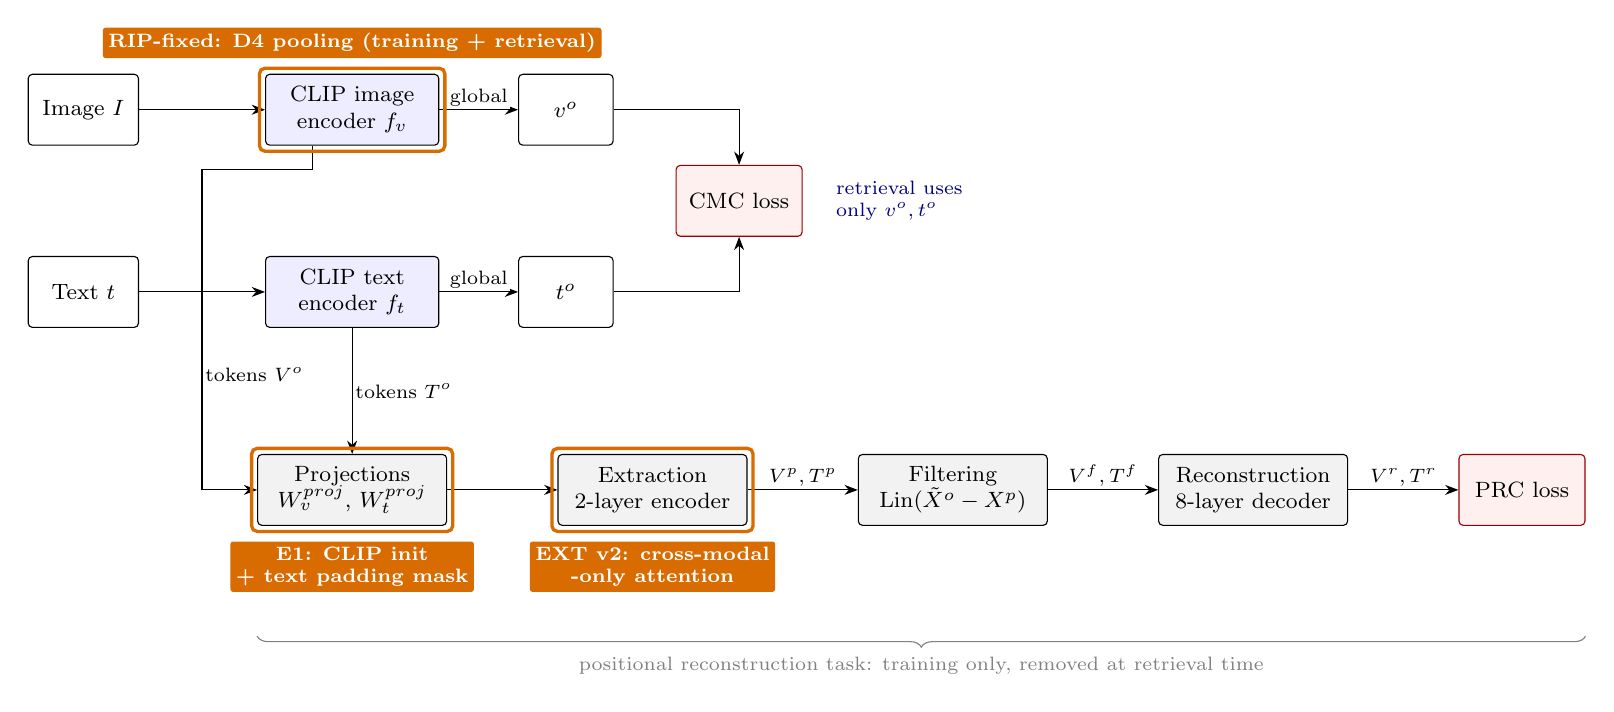
\begin{tikzpicture}[
  font=\footnotesize, >=Stealth, node distance=5mm,
  box/.style={draw, rounded corners=1.5pt, align=center, minimum height=9mm, inner sep=3pt, fill=white},
  enc/.style={box, fill=blue!7, minimum width=22mm},
  mod/.style={box, fill=gray!10, minimum width=24mm},
  modmark/.style={draw=orange!85!black, very thick, rounded corners=2pt},
  tag/.style={fill=orange!85!black, text=white, font=\scriptsize\bfseries, rounded corners=1pt, inner sep=2pt, align=center},
  lossb/.style={box, fill=red!6, draw=red!60!black, minimum width=16mm},
  lab/.style={font=\scriptsize, fill=white, inner sep=1pt}
]
% inputs and encoders
\node[box, minimum width=14mm] (img) {Image $I$};
\node[box, minimum width=14mm, below=14mm of img] (txt) {Text $t$};
\node[enc, right=16mm of img] (venc) {CLIP image\\encoder $f_v$};
\node[enc, right=16mm of txt] (tenc) {CLIP text\\encoder $f_t$};
\draw[->] (img) -- (venc);
\draw[->] (txt) -- (tenc);
% global path (used for retrieval)
\node[box, right=10mm of venc, minimum width=12mm] (vg) {$v^{o}$};
\node[box, right=10mm of tenc, minimum width=12mm] (tg) {$t^{o}$};
\draw[->] (venc) -- node[lab, above] {global} (vg);
\draw[->] (tenc) -- node[lab, above] {global} (tg);
\node[lossb] (cmc) at ($(vg)!0.5!(tg) + (22mm,0)$) {CMC loss};
\draw[->] (vg) -| (cmc);
\draw[->] (tg) -| (cmc);
\node[font=\scriptsize, text=blue!50!black, align=left, right=3mm of cmc] {retrieval uses\\only $v^{o}, t^{o}$};
% token path (training only)
\node[mod, below=16mm of tenc] (proj) {Projections\\$W_v^{proj}$, $W_t^{proj}$};
\node[mod, right=14mm of proj] (ext) {Extraction\\2-layer encoder};
\node[mod, right=14mm of ext] (fil) {Filtering\\$\mathrm{Lin}(\tilde X^{o}-X^{p})$};
\node[mod, right=14mm of fil] (rec) {Reconstruction\\8-layer decoder};
\node[lossb, right=14mm of rec] (prc) {PRC loss};
\draw[->] ($(venc.south)+(-5mm,0)$) -- ++(0,-3mm) -| ($(proj.west)+(-7mm,0)$) node[lab, pos=0.82, right] {tokens $V^{o}$} -- (proj.west);
\draw[->] (tenc) -- node[lab, right] {tokens $T^{o}$} (proj);
\draw[->] (proj) -- (ext);
\draw[->] (ext) -- node[lab, above] {$V^{p}, T^{p}$} (fil);
\draw[->] (fil) -- node[lab, above] {$V^{f}, T^{f}$} (rec);
\draw[->] (rec) -- node[lab, above] {$V^{r}, T^{r}$} (prc);
% modification marks
\node[modmark, fit=(venc), inner sep=2pt] (m1) {};
\node[tag, above=1mm of m1] {RIP-fixed: D4 pooling (training + retrieval)};
\node[modmark, fit=(proj), inner sep=2pt] (m2) {};
\node[tag, below=1mm of m2] {E1: CLIP init\\+ text padding mask};
\node[modmark, fit=(ext), inner sep=2pt] (m3) {};
\node[tag, below=1mm of m3] {EXT v2: cross-modal\\-only attention};
% train-only bracket
\draw[decorate, decoration={brace, amplitude=4pt, mirror}, gray]
  ([yshift=-14mm]proj.south west) -- ([yshift=-14mm]prc.south east)
  node[midway, below=4pt, gray, font=\scriptsize] {positional reconstruction task: training only, removed at retrieval time};
\end{tikzpicture}
}
\caption{PR-CLIP training pipeline (released code). Orange boxes mark where our A3 modifications act. Extraction, filtering, and reconstruction run only during training. RIP-fixed changes the image embedding used both in training and at retrieval time.}
\label{fig:arch}
\end{figure*}


\begin{table}[t]
\centering
\caption{Differences between the PR-CLIP paper and the released code (commit \texttt{242fba6}).}
\label{tab:audit}
\scriptsize
\setlength{\tabcolsep}{3pt}
\begin{tabular}{@{}lll@{}}
\toprule
Item & Paper & Released code \\
\midrule
Loss & $0.01\,\mathcal{L}_{CMC}+\mathcal{L}_{PRC}$ & $(1.5\,\mathcal{L}_{NCE}+\mathrm{MSE}_{pool})/4$ \\
LR, RSICD & $5\mathrm{e}{-5}$ & $5\mathrm{e}{-6}$ \\
LR, RSITMD & $5\mathrm{e}{-6}$ & $5\mathrm{e}{-5}$ \\
Selection & train / val / test & \texttt{best.pt} on test CSV \\
RSICD val & separate split & = test file (same SHA-256) \\
Checkpoint & released & link gives image archive \\
Tokens & -- & no \texttt{return\_hidden} in OpenCLIP 2.20 \\
AMP branch & -- & no \texttt{zero\_grad()}: grad $=$ NaN, no update \\
\bottomrule
\end{tabular}
\end{table}

% ===========================================================================
\section{Investigated Modifications}

\subsection{Notation}
Table~\ref{tab:notation} defines the labels used in the rest of the report.

\begin{table}[t]
\centering
\caption{Labels and abbreviations}
\label{tab:notation}
\footnotesize
\begin{tabular}{@{}p{0.23\columnwidth}p{0.70\columnwidth}@{}}
\toprule
Label & Meaning \\
\midrule
RET-2 & Training set of PR-CLIP: RSICD + RSITMD after RemoteCLIP de-duplication; 13{,}092 images, 65{,}460 pairs. \\
RET-2 ckpt & GeoRSCLIP RS5M ViT-B/32 checkpoint fine-tuned on RET-2 (\texttt{RS5M\_ViT-B-32\_RET-2.pt}) \cite{zhang2024georsclip}. \\
A3 & Our controlled module study: same code, data, seed list and hyper-parameters; only module flags change. \\
B1 & A3 baseline: released PR-CLIP code, no added module. \\
RIP-fixed & D4 rotation-invariant pooling of image embeddings, used in training and retrieval (Sec.~\ref{sec:rip}). \\
E1 & Text padding mask in extraction + CLIP-initialised projections $W^{proj}$ (Sec.~\ref{sec:e1}). \\
EXT v2 & Extraction encoder restricted to cross-modal attention (Sec.~\ref{sec:ext2}). \\
R2 / R4 / R3 & RIP-fixed / RIP-fixed+E1 / RIP-fixed+E1+EXT v2. \\
Epoch 0 & Evaluation of the RET-2 ckpt before any training. \\
\bottomrule
\end{tabular}
\end{table}

\subsection{RIP-fixed: D4 Rotation-Invariant Pooling}
\label{sec:rip}
Let $G_{D4}$ be the eight transforms of a square image: rotations by $0^\circ, 90^\circ, 180^\circ, 270^\circ$ and the same rotations after a horizontal flip. For image $I$,
\begin{equation}
\bar v = \frac{1}{8}\sum_{g\in G_{D4}} \frac{f_v(g(I))}{\lVert f_v(g(I))\rVert_2},\qquad
v_{D4} = \frac{\bar v}{\lVert \bar v\rVert_2}\,\lVert f_v(I)\rVert_2 .
\label{eq:rip}
\end{equation}
The direction of $v_{D4}$ is the same for all eight transformed versions of $I$, and its norm equals that of the original embedding, so the logit scale keeps its meaning. During training only the identity branch keeps gradients; the other seven run without gradient tracking. The same pooling is used when computing retrieval embeddings. ``Fixed'' refers to this fixed, parameter-free averaging.

\emph{Cost.} Each image needs eight forward passes of $f_v$. For T2I retrieval the image gallery is encoded once offline, so the query cost does not change. For I2T retrieval the query image is encoded eight times. Text encoding is unchanged. RIP-fixed can be harmful when the caption depends on absolute direction (``north of the river''); RSICD captions rarely do this.

\subsection{E1: Padding-Aware, CLIP-Initialised Extraction}
\label{sec:e1}
In the released code all 77 text positions, including padding after the end-of-text token, enter the extraction encoder. E1 adds a key-padding mask so that padding tokens are ignored. It also initialises $W_v^{proj}$ ($768\to512$) with CLIP's visual projection and $W_t^{proj}$ ($512\to512$) with CLIP's text projection, with zero bias, instead of random weights. E1 adds no parameters.

\subsection{EXT v2: Cross-Modal-Only Extraction}
\label{sec:ext2}
EXT~v2 keeps the original 2-layer encoder and its weights but applies an attention mask that blocks image--image and text--text attention. The self-attention layers then act as bidirectional cross attention, so every extracted feature is built only from the other modality. This matches the role the extraction output plays in filtering, where it is subtracted as ``information shared with the other modality''. EXT~v2 adds no parameters.

\subsection{Other Explored Variants}
Before A3 we explored three variants, each in its own setup. (i) \emph{Dual residual adapter}: an identity-initialised bottleneck MLP $x' = x + f_\theta(x)$ on the image and text retrieval embeddings, trained with a 100$\times$ learning rate. (ii) \emph{BRCR} (bidirectional reliability-aware cross-modal reconstruction): token-weighted pooling $z=\sum_i \alpha_i h_i$ in the reconstruction loss, a text padding mask, bidirectional decoder attention, detached targets, and optionally a sum instead of mean loss reduction. (iii) \emph{Modified extraction}: modality-type embeddings, pre-layer normalisation, GELU, and a text padding mask. These variants are reported in Sec.~\ref{sec:explore} but were not run under the A3 protocol.

% ===========================================================================
\section{Experimental Setup}
\label{sec:setup}

\subsection{Datasets and Splits}
We train on RET-2 and test on RSICD (1{,}093 images, 5{,}465 captions) \cite{lu2018rsicd} and RSITMD (452 images, 2{,}260 captions) \cite{yuan2022amfmn}, using the CSV files released with PR-CLIP. No test image appears in the RET-2 training file.

The released split has a problem for model selection. \texttt{rsicd\_val.csv} is byte-identical to \texttt{rsicd\_test.csv} (same SHA-256), and 733 of the 856 images in \texttt{rsitmd\_val.csv} also appear in RET-2 training. We therefore hold out 10\% of RET-2 \emph{images} (1{,}311 images, 6{,}555 pairs; stratified by scene name, seed 0) as a validation split, and train on the remaining 11{,}781 images. All five captions of an image stay on the same side. The script and SHA-256 manifest are in the repository.

\subsection{Initialization}
All A3 runs start from the RET-2 ckpt. Some earlier runs start from the original OpenAI CLIP ViT-B/32 weights; these are labelled ``CLIP'' and are not comparable with RET-2 runs.

\subsection{Training Configuration}
The A3 setup is: 1 epoch, batch size 16, learning rate $2\times10^{-7}$, 100 warm-up steps, weight decay 0.5, maximum gradient norm 50, AMP, ViT-B/32 at $224\times224$. Seeds 1, 2 and 3 are used for every trained configuration. Hyper-parameters are not tuned per module. All A3 runs use the AMP fix described in Sec.~\ref{sec:background} and were run on one RTX 4060 Laptop GPU (8\,GB); one epoch takes about 15 minutes for B1 and 23 minutes with RIP-fixed.

\subsection{Evaluation Protocol}
\begin{itemize}
\item \textbf{Epoch 0} is the RET-2 ckpt evaluated directly. It is deterministic, so it needs one run per configuration.
\item \textbf{Epoch 1} is evaluated on validation and test after one epoch, for each seed.
\item \textbf{Validation-selected}: for each seed, the epoch (0 or 1) with the higher validation mR is chosen, and only that model's test result is reported. The test set is never used to choose an epoch or checkpoint.
\item We report mean $\pm$ sample standard deviation over seeds.
\item Inference time IT(s) is the wall-clock time to encode all test images and captions and compute the ranking, measured on the same GPU for every configuration.
\end{itemize}

\subsection{Metrics}
For $K\in\{1,5,10\}$, R@$K$ is the share of queries whose ground-truth match is in the top $K$. With five captions per image, an I2T query counts as correct if any of its captions is in the top $K$. Mean Recall is
\begin{equation}
\mathrm{mR} = \frac{1}{6}\sum_{K\in\{1,5,10\}}\big(R_{I2T}@K + R_{T2I}@K\big).
\end{equation}
All values are percentages.

\subsection{Implementation and Reproducibility}
All A3 changes are in \texttt{prclip\_patches/} of our repository: \texttt{apply\_patches.py} applies them to the authors' code at commit \texttt{242fba6}, and modules are switched only by the environment variables \texttt{PRCLIP\_RIP}, \texttt{PRCLIP\_E1} and \texttt{PRCLIP\_EXT2}. Unit tests in \texttt{tests/} check D4 invariance, norm preservation, gradient flow, and masking. The notebook \texttt{A3\_MultiSeed\_Colab.ipynb} (Colab) and \texttt{RUN\_A3\_GPU.bat} (local Windows GPU) run the full protocol and writes every evaluation to \texttt{metrics.jsonl}; \texttt{aggregate\_results.py} produces Table~\ref{tab:a3}. Logs of earlier runs are stored in \texttt{results/legacy/}.

% ===========================================================================
\section{Results}

\subsection{Reference Results}
Table~\ref{tab:published} lists published RSICD results and our evaluation of the RET-2 ckpt. Our evaluation of the RET-2 ckpt (38.86\%) agrees with the GeoRSCLIP result reported in the PR-CLIP paper (38.87\%): the three T2I values are identical, and I2T R@1 and R@5 differ by less than 0.3 points, which we attribute to image decoding and resizing in different library versions. On RSITMD all six values equal the published GeoRSCLIP numbers (51.81\%). This is the same checkpoint, not a reproduction of PR-CLIP. It is 0.37 points below PR-CLIP on RSICD and 0.60 points below on RSITMD.

\begin{table*}[t]
\centering
\caption{Published RSICD results \cite{guan2025prclip} and our evaluation of the starting checkpoint. Values in \%.}
\label{tab:published}
\footnotesize
\begin{tabular}{@{}llccccccc@{}}
\toprule
Method & Training data & I2T R@1 & I2T R@5 & I2T R@10 & T2I R@1 & T2I R@5 & T2I R@10 & mR \\
\midrule
AMFMN \cite{yuan2022amfmn} & RSICD & 5.39 & 15.08 & 23.40 & 4.90 & 18.28 & 31.44 & 16.42 \\
GaLR \cite{yuan2022galr} & RSICD & 6.59 & 19.85 & 31.04 & 4.69 & 19.48 & 32.13 & 18.96 \\
MTGFE \cite{zhang2023mtgfe} & RSICD & 15.28 & 37.05 & 51.60 & 8.67 & 27.56 & 43.92 & 30.68 \\
PE-RSITR \cite{yuan2023pe} & RSICD & 14.13 & 31.51 & 44.78 & 11.63 & 33.92 & 50.73 & 31.12 \\
RemoteCLIP \cite{liu2024remoteclip} & RET-3+DET-10+SEG-4 & 17.02 & 37.97 & 51.51 & 13.71 & 37.11 & 54.25 & 35.26 \\
GeoRSCLIP \cite{zhang2024georsclip} & RS5M+RET-2 & 21.13 & 41.72 & 55.63 & 15.59 & 41.19 & 57.99 & 38.87 \\
PR-CLIP \cite{guan2025prclip} & RET-2 & 22.32 & 40.81 & 55.90 & 16.47 & 41.74 & 58.12 & 39.23 \\
\midrule
RET-2 ckpt, our evaluation & RS5M+RET-2 & 20.86 & 41.90 & 55.63 & 15.59 & 41.24 & 57.95 & 38.86 \\
\bottomrule
\end{tabular}
\end{table*}

\subsection{RIP-fixed Without Training}
Table~\ref{tab:ep0} reports the RET-2 ckpt at epoch 0 with and without RIP-fixed. These evaluations involve no training and no random choice, so repeated runs give identical numbers; we re-ran each one twice to confirm this. On RSICD, RIP-fixed raises mR from 38.86\% to 39.70\% (+0.84). The gain comes from I2T R@5/R@10 and all three T2I recalls, while I2T R@1 drops slightly (20.86 to 20.59). The result is 0.47 points above the published PR-CLIP result, without positional reconstruction or training. It agrees with the preliminary A3 run (38.89\% and 39.66\%). After one epoch of fine-tuning, both configurations dropped (to 38.72\% and 39.09\%).

On RSITMD the picture is different: mR moves from 51.81\% to 51.88\% (+0.07), and RIP-fixed stays below PR-CLIP (52.41\%). Here seed noise does not apply, but the test set is finite. A paired bootstrap over test images (2{,}000 resamples, each image kept with its five captions) gives a 95\% interval of [+0.29, +1.42] points for the RSICD gain (resampling std 0.29; gain $\le 0$ in 0.1\% of resamples) and [-0.77, +0.87] for RSITMD (gain $\le 0$ in 43.1\%).

One caution remains: RIP-fixed was chosen after the team had seen RSICD test results, so the RSICD gain is partly a selection effect. RSITMD, which was not used to design the module, shows almost no gain. The validation-selected, three-seed results after training are given in Sec.~\ref{sec:a3}.

\begin{table*}[t]
\centering
\caption{RET-2 ckpt evaluated without training (epoch 0). Deterministic (two identical runs). IT(s): wall-clock time to encode all test images, measured on 2 CPU threads; text encoding is the same for both rows and is excluded. Logs: \texttt{results/a3/epoch0\_*}.}
\label{tab:ep0}
\footnotesize
\begin{tabular}{@{}llcccccccc@{}}
\toprule
Test set & Configuration & I2T R@1 & I2T R@5 & I2T R@10 & T2I R@1 & T2I R@5 & T2I R@10 & mR & IT(s) \\
\midrule
\multirow{3}{*}{RSICD} & B1 (single pass) & 20.86 & 41.90 & 55.63 & 15.59 & 41.24 & 57.95 & 38.86 & 50 \\
 & RIP-fixed (8 passes) & 20.59 & 43.28 & 57.37 & 15.72 & 42.32 & 58.90 & 39.70 & 402 \\
 & PR-CLIP (published) & 22.32 & 40.81 & 55.90 & 16.47 & 41.74 & 58.12 & 39.23 & -- \\
\midrule
\multirow{3}{*}{RSITMD} & B1 (single pass) & 32.30 & 53.32 & 67.92 & 25.04 & 57.88 & 74.38 & 51.81 & 20 \\
 & RIP-fixed (8 passes) & 32.52 & 53.10 & 66.81 & 25.40 & 58.14 & 75.31 & 51.88 & 167 \\
 & PR-CLIP (published) & 32.74 & 54.65 & 66.59 & 27.43 & 58.36 & 74.69 & 52.41 & -- \\
\bottomrule
\multicolumn{10}{@{}p{0.95\textwidth}@{}}{Paired bootstrap 95\% interval of the mR gain (RIP-fixed $-$ B1): RSICD [+0.29, +1.42], RSITMD [-0.77, +0.87]. With the authors' evaluation code on an RTX 4060 Laptop GPU the same checkpoint gives 38.89/39.67 (RSICD) and 51.81/51.89 (RSITMD) for B1/RIP-fixed, with total inference time 21.3\,s vs.\ 35.5\,s on RSICD (PR-CLIP reports 3.95\,s on an RTX 4090). On CPU RIP-fixed needs 8.1$\times$ the image-encoding time.}
\end{tabular}
\end{table*}

\subsection{Controlled A3 Module Study}
\label{sec:a3}
Table~\ref{tab:a3} lists the A3 results. The upper block repeats the preliminary single-seed runs from our earlier notebooks, where the epoch was chosen on RSICD test. The lower block is the re-run under the protocol of Sec.~\ref{sec:setup}: the same patched code for every configuration, training on the RET-2 training split, seeds 1--3, and model selection on the held-out validation split. For every configuration and seed, validation mR rose after one epoch (B1: 55.02 to 56.13--56.59\%; R2 and R3: 56.79 to 57.81--58.02\%), so the validation rule always selected epoch~1. The lower block therefore reports epoch-1 test results.

RIP-fixed improves the matched baseline on every seed and on both test sets. The paired per-seed gain is $+0.34 \pm 0.09$ points on RSICD (seeds: $+0.44, +0.31, +0.27$) and $+0.66 \pm 0.17$ on RSITMD ($+0.63, +0.50, +0.84$); a paired $t$-test gives $p=0.02$ in both cases. The seed spread of B1 itself is small (std 0.16 and 0.26). E1 and EXT~v2 on top of RIP-fixed change mR by $+0.01 \pm 0.06$ (RSICD) and $-0.01 \pm 0.07$ (RSITMD), so they have no measurable effect in this setup. The preliminary run reached 39.09--39.11\% on RSICD; the re-run gives 38.68--39.17\% across seeds, so the earlier numbers were at the upper end of the seed range.

Training and test disagree. One epoch lowers RSICD test mR for both B1 ($38.89 \to 38.56$) and RIP-fixed ($39.67 \to 38.90$), while it raises RSITMD for RIP-fixed ($51.89 \to 52.29$). The validation split is drawn from RET-2, which mixes RSICD-like and RSITMD-like images, so validation-based selection does not protect the RSICD result here. The best validation-selected results (38.91\% on RSICD, 52.29\% on RSITMD) remain 0.32 and 0.12 points below PR-CLIP; seed~1 of R2 and R3 exceeds PR-CLIP on RSITMD (52.47 and 52.52\%), but the three-seed mean does not.

\begin{table*}[t]
\centering
\caption{Controlled A3 study (1 epoch, batch 16, lr $2\times10^{-7}$, RET-2 init). Upper block: preliminary runs (seed 1, epoch chosen on RSICD test, no validation). Lower block: re-run with the released protocol, seeds 1--3, mean $\pm$ std over seeds; validation selected epoch 1 for every run. $\Delta$: paired per-seed mR difference to B1 (mean $\pm$ std). Logs: \texttt{results/a3/raw\_logs/}.}
\label{tab:a3}
\scriptsize
\setlength{\tabcolsep}{3.2pt}
\begin{tabular}{@{}llcccccccccc@{}}
\toprule
Run & Test & $n$ & I2T R@1 & I2T R@5 & I2T R@10 & T2I R@1 & T2I R@5 & T2I R@10 & mR & $\Delta$ \\
\midrule
PR-CLIP (published) & RSICD & -- & 22.32 & 40.81 & 55.90 & 16.47 & 41.74 & 58.12 & 39.23 & \\
PR-CLIP (published) & RSITMD & -- & 32.74 & 54.65 & 66.59 & 27.43 & 58.36 & 74.69 & 52.41 & \\
\midrule
B1 baseline (prelim.) & RSICD & 1 & 20.31 & 40.99 & 53.80 & 16.40 & 42.01 & 58.79 & 38.72 & -- \\
R2 RIP-fixed (prelim.) & RSICD & 1 & 19.95 & 41.08 & 55.44 & 16.32 & 42.16 & 59.58 & 39.09 & +0.37 \\
R4 RIP+E1 (prelim.) & RSICD & 1 & 19.95 & 41.26 & 55.35 & 16.43 & 42.07 & 59.52 & 39.10 & +0.38 \\
R3 RIP+E1+EXT v2 (prelim.) & RSICD & 1 & 20.04 & 40.99 & 55.72 & 16.40 & 42.16 & 59.36 & 39.11 & +0.39 \\
\midrule
B1 baseline & RSICD & 3 & 20.10$\pm$0.05 & 41.02$\pm$0.38 & 54.16$\pm$0.33 & 16.04$\pm$0.24 & 41.55$\pm$0.25 & 58.51$\pm$0.19 & 38.56$\pm$0.16 & -- \\
R2 RIP-fixed & RSICD & 3 & 20.28$\pm$0.42 & 41.29$\pm$0.53 & 54.65$\pm$0.30 & 15.91$\pm$0.11 & 42.08$\pm$0.24 & 59.19$\pm$0.37 & 38.90$\pm$0.25 & +0.34$\pm$0.09 \\
R3 RIP+E1+EXT v2 & RSICD & 3 & 20.34$\pm$0.32 & 41.26$\pm$0.48 & 54.65$\pm$0.14 & 15.90$\pm$0.06 & 42.08$\pm$0.22 & 59.23$\pm$0.32 & 38.91$\pm$0.21 & +0.35$\pm$0.05 \\
\midrule
B1 baseline & RSITMD & 3 & 32.52$\pm$0.80 & 52.29$\pm$0.68 & 66.45$\pm$0.89 & 25.03$\pm$0.28 & 58.14$\pm$0.28 & 75.38$\pm$0.22 & 51.64$\pm$0.26 & -- \\
R2 RIP-fixed & RSITMD & 3 & 33.11$\pm$0.71 & 53.61$\pm$0.51 & 66.67$\pm$0.46 & 26.03$\pm$0.25 & 58.48$\pm$0.34 & 75.86$\pm$0.31 & 52.29$\pm$0.16 & +0.66$\pm$0.17 \\
R3 RIP+E1+EXT v2 & RSITMD & 3 & 32.97$\pm$0.39 & 53.54$\pm$0.58 & 66.74$\pm$0.56 & 26.05$\pm$0.18 & 58.54$\pm$0.48 & 75.86$\pm$0.31 & 52.28$\pm$0.22 & +0.64$\pm$0.13 \\
\bottomrule
\end{tabular}
\end{table*}

\subsection{Sensitivity to Optimization and Initialization}
Table~\ref{tab:sens} gives earlier runs that vary the learning rate, number of epochs, seed, batch size and initialization. Every fine-tuning run from the RET-2 ckpt ended below the checkpoint itself (38.86\%). With learning rate $5\times10^{-6}$ and seed 1, mR fell from 38.15\% after one epoch to 37.51\% after two and 36.96\% after three. A 20-epoch RET-2 run peaked at 36.77\% (epoch 15) and ended at 36.48\%. Runs from OpenAI CLIP weights stayed between 34.27\% and 36.86\%. These runs selected the best epoch on the test set, so the ``best epoch'' numbers are optimistic; the trend, however, is consistent. Without training-loss and validation curves we cannot tell whether the drop is overfitting or drift away from the RS5M representation.

\begin{table}[t]
\centering
\caption{Earlier runs on RSICD test (mR, \%). lr: learning rate; ep: epochs; best ep.\ was chosen on test. Log: \checkmark{} = notebook output in repository; \pend{} = log to be uploaded.}
\label{tab:sens}
\footnotesize
\begin{tabular}{@{}lllcc@{}}
\toprule
Init & Setting & Seed & mR & Log \\
\midrule
RET-2 & no training & -- & 38.86 & \checkmark \\
RET-2 & 1 ep, lr $2\mathrm{e}{-7}$ & 1 & 38.72 & \pend \\
RET-2 & 1 ep, lr $2\mathrm{e}{-7}$ & -- & 38.70 & \pend \\
RET-2 & 1 ep, lr $5\mathrm{e}{-6}$ & 1 & 38.15 & \pend \\
RET-2 & 1 ep, lr $1\mathrm{e}{-6}$ & -- & 38.11 & \pend \\
RET-2 & 1 ep, lr $5\mathrm{e}{-6}$ & 2 & 37.75 & \pend \\
RET-2 & 2 ep, lr $5\mathrm{e}{-6}$ & 1 & 37.51 & \pend \\
RET-2 & 3 ep, lr $5\mathrm{e}{-6}$ & 1 & 36.96 & \pend \\
RET-2 & 20 ep, best ep.\ 15 & -- & 36.77 & \pend \\
RET-2 & 20 ep, final & -- & 36.48 & \pend \\
CLIP & 20 ep, best ep.\ 17 & 0 & 36.86 & \pend \\
CLIP & 20 ep, best ep.\ 9 & 1 & 36.33 & \pend \\
CLIP & 20 ep, best ep.\ 11 & 3 & 35.31 & \pend \\
CLIP & batch 64, 20 ep, best ep.\ 5 & -- & 34.27 & \pend \\
\bottomrule
\end{tabular}
\end{table}

\subsection{Exploratory Variants}
\label{sec:explore}
Table~\ref{tab:explore} lists the variants tested before A3. None exceeded the RET-2 ckpt. Turning on every BRCR switch, including sum-reduced loss, gave the lowest result (37.97\%); because several switches changed at once, the drop cannot be attributed to one of them. The modified extraction module reached 38.74\% alone, in line with the very small extraction effect in A3. These variants used setups that differ from A3 (for example the adapter's 100$\times$ learning rate), so they should not be ranked against Table~\ref{tab:a3}.

\begin{table}[t]
\centering
\caption{Exploratory variants on RSICD test (1 epoch, batch 16, lr $2\mathrm{e}{-7}$, RET-2 init, seed 1).}
\label{tab:explore}
\footnotesize
\begin{tabular}{@{}lcl@{}}
\toprule
Variant & mR & Log \\
\midrule
RET-2 ckpt (no training) & 38.86 & \checkmark{} \texttt{epoch0} \\
Modified extraction & 38.74 & \checkmark{} \texttt{PR\_CLIP\_(2)} \\
Dual residual adapter & 38.69 & \pend \\
BRCR (mask, bidir, rel, detach) & 38.68 & \checkmark{} \texttt{PR\_CLIP\_v4\_BRCR} \\
BRCR, all switches (+ sum loss) & 37.97 & \pend \\
\bottomrule
\end{tabular}
\end{table}


\subsection{Objective Ablation from OpenAI CLIP}
\label{sec:objective}
To see how the reconstruction term itself behaves, we ran a separate small study with an independent re-implementation of Eqs.~(3)--(13) (repository \texttt{phamhongnhattan-boop/PR-CLIP}, folder \texttt{repro/}). It starts from OpenAI CLIP ViT-B/32 (not the RET-2 ckpt) and trains for 100 steps on 200 RET-2 pairs (batch 2, lr $5\times10^{-6}$, seed 3407). The model is chosen on \texttt{rsitmd\_val.csv}, and the test sets are evaluated once afterwards (Table~\ref{tab:objective}). With this tiny budget, both objectives that include reconstruction destroyed retrieval (mR 1.41\% and 0.75\% on RSITMD val), while the contrastive term alone improved on CLIP. This does not show that PRC is useless at full scale: batch size, initialization and training length are far from the paper. It does show that the reconstruction loss can dominate the update when the contrastive weight is 0.01, which supports keeping the reconstruction branch light in our A3 setup.

\begin{table}[t]
\centering
\caption{Objective ablation, OpenAI CLIP init, 100 steps on 200 RET-2 pairs, one seed. mR in \%. Logs: \texttt{results/objective\_ablation/}.}
\label{tab:objective}
\footnotesize
\begin{tabular}{@{}lccc@{}}
\toprule
Objective & RSITMD val & RSITMD test & RSICD test \\
\midrule
OpenAI CLIP, no training & 16.77 & 24.23 & 15.69 \\
$0.01\,$CMC $+$ PRC (paper) & 1.41 & -- & -- \\
Released-style pooled MSE & 0.75 & -- & -- \\
$0.01\,$CMC only & \textbf{18.59} & \textbf{25.10} & \textbf{17.31} \\
\bottomrule
\end{tabular}
\end{table}

% ===========================================================================
\section{Discussion}
\textbf{The starting checkpoint dominates.} The RET-2 ckpt already gives 38.86\% on RSICD and 51.81\% on RSITMD, within 0.4 and 0.6 points of PR-CLIP. On RSICD every fine-tuning setting we tried moved away from it; on RSITMD only fine-tuning with RIP-fixed improved on it. Under a small budget, keeping the pretrained representation was usually more effective than adapting it.

\textbf{RIP-fixed is the only change with a reliable effect.} After one epoch it improves the baseline on every seed and on both test sets ($+0.34$ and $+0.66$ points, $p=0.02$). Without training, its gain was larger on RSICD ($+0.84$) but absent on RSITMD ( +0.07 points, within resampling noise). Training thus moves the gain from RSICD towards RSITMD; RSICD contains many scene-level captions without direction words, while RSITMD captions are longer and describe object relations more often, which may make orientation pooling less useful there; we have not tested this explanation. Because the pooling acts on the embeddings used at retrieval time, it can help without any training; during training the backbone also adapts to the pooled embedding, which may explain the larger RSITMD gain after one epoch. Averaging over D4 also makes the gallery embeddings of rotated copies of a scene identical, which fits nadir imagery where orientation is arbitrary. The cost is eight image-encoder passes per image; for T2I search this is an offline indexing cost only.

\textbf{Extraction changes have little effect in this setup.} Extraction only shapes gradients, and one epoch at a very small learning rate gives it little room to change the backbone. A fair test of E1 and EXT~v2 would need longer training with the paper's objective and batch size.

\textbf{Seeds and selection matter.} Across three seeds the B1 result varies by up to 0.3 points on RSICD and 0.5 points on RSITMD, which is why single-seed gains of a few hundredths (R2 vs.\ R3 vs.\ R4) carry no information. Validation on held-out RET-2 images always preferred the trained model, yet on RSICD the untrained checkpoint scored higher on test; a validation split that matches each test domain would be needed to select between them fairly.

% ===========================================================================
\section{Limitations}
\begin{itemize}
\item We did not retrain PR-CLIP with the paper's objective, batch size 160 and 20 epochs; the released code's objective also differs from the paper's equation. No number here is a full reproduction of 39.23\%.
\item The A3 study trains for one epoch with three seeds on a single RTX 4060 Laptop GPU; longer training with the paper's objective and batch size may change the ranking. R4 (RIP+E1) was not re-run, since R3 already shows that E1 and EXT~v2 together have no effect.
\item The epoch-0 results are deterministic, but RIP-fixed was designed after seeing RSICD test results; its gain does not hold on RSITMD.
\item The validation split is carved from RET-2, so A3 runs in the new protocol train on 10\% fewer images than the preliminary runs, and it mixes RSICD- and RSITMD-like images, so it did not predict the RSICD test trend.
\item RIP-fixed is evaluated only on RSICD and RSITMD; it may hurt captions with absolute directions, which we have not measured separately. Inference time was measured on a laptop GPU (RTX 4060) and on CPU, not on the RTX 4090 used by the paper.
\item The exploratory variants were not run under the A3 protocol and lack a complete factorial ablation.
\item The objective ablation (Table~\ref{tab:objective}) uses 200 pairs, batch 2 and one seed, so it only shows behaviour at a very small budget.
\end{itemize}

% ===========================================================================
\section{Conclusion}
We studied PR-CLIP starting from the public RET-2 checkpoint under a small training budget. The checkpoint alone reaches 38.86\% mR on RSICD, and every fine-tuning run we tried ended below it on that test set. Among parameter-free changes, D4 rotation-invariant pooling was the only one with a noticeable effect: with no training it gives 39.70\% on RSICD (+0.84, bootstrap 95\% interval [+0.29, +1.42]), above the published PR-CLIP result, at the cost of eight image-encoder passes per image. On RSITMD the same change gives only +0.07 points without training. After one epoch with three seeds, RIP-fixed improves the matched baseline on every seed on both test sets ($+0.34$ on RSICD, $+0.66$ on RSITMD), but the validation-selected models (38.91\% and 52.29\%) stay below PR-CLIP. The extraction variants E1 and EXT~v2 changed mR by about $\pm$0.01 points. We release the module patch (including a fix for the released mixed-precision training loop), a validation split that fixes the val/test overlap in the public CSV files, all logs, and scripts that reproduce every table. Future work should run PR-CLIP with the paper's objective and configuration, test RIP-fixed on direction-dependent captions, and replace uniform D4 averaging with learned aggregation \cite{shanmugam2021tta}.

\section*{Code Availability}
Code, patches, notebooks and logs: \url{https://github.com/phamhongnhattan-boop/PR-CLIP-Improved}. Authors' PR-CLIP code: \url{https://github.com/ADMIS-TONGJI/PR-CLIP} (commit \texttt{242fba6}).

% ===========================================================================
\begin{thebibliography}{99}
\footnotesize

\bibitem{guan2025prclip}
J.~Guan, Y.~Shu, W.~Li, Z.~Song, and Y.~Zhang, ``PR-CLIP: Cross-modal positional reconstruction for remote sensing image--text retrieval,'' \emph{Remote Sens.}, vol.~17, no.~13, Art.~no.~2117, 2025, doi: 10.3390/rs17132117.

\bibitem{prclipcode}
ADMIS-TONGJI, ``PR-CLIP,'' GitHub repository, 2025. [Online]. Available: \url{https://github.com/ADMIS-TONGJI/PR-CLIP}

\bibitem{itra}
D.~Chen, ``ITRA,'' GitHub repository. [Online]. Available: \url{https://github.com/ChenDelong1999/ITRA}

\bibitem{radford2021clip}
A.~Radford \emph{et~al.}, ``Learning transferable visual models from natural language supervision,'' in \emph{Proc. 38th Int. Conf. Mach. Learn. (ICML)}, 2021, pp.~8748--8763.

\bibitem{dosovitskiy2021vit}
A.~Dosovitskiy \emph{et~al.}, ``An image is worth 16x16 words: Transformers for image recognition at scale,'' in \emph{Proc. Int. Conf. Learn. Represent. (ICLR)}, 2021.

\bibitem{lu2018rsicd}
X.~Lu, B.~Wang, X.~Zheng, and X.~Li, ``Exploring models and data for remote sensing image caption generation,'' \emph{IEEE Trans. Geosci. Remote Sens.}, vol.~56, no.~4, pp.~2183--2195, 2018.

\bibitem{yuan2022amfmn}
Z.~Yuan \emph{et~al.}, ``Exploring a fine-grained multiscale method for cross-modal remote sensing image retrieval,'' \emph{IEEE Trans. Geosci. Remote Sens.}, vol.~60, pp.~1--19, 2022.

\bibitem{yuan2022galr}
Z.~Yuan \emph{et~al.}, ``Remote sensing cross-modal text-image retrieval based on global and local information,'' \emph{IEEE Trans. Geosci. Remote Sens.}, vol.~60, pp.~1--16, 2022.

\bibitem{faghri2018vsepp}
F.~Faghri, D.~J. Fleet, J.~R. Kiros, and S.~Fidler, ``VSE++: Improving visual-semantic embeddings with hard negatives,'' in \emph{Proc. Brit. Mach. Vis. Conf. (BMVC)}, 2018.

\bibitem{lee2018scan}
K.-H. Lee, X.~Chen, G.~Hua, H.~Hu, and X.~He, ``Stacked cross attention for image-text matching,'' in \emph{Proc. Eur. Conf. Comput. Vis. (ECCV)}, 2018, pp.~201--216.

\bibitem{pan2023swan}
J.~Pan, Q.~Ma, and C.~Bai, ``Reducing semantic confusion: Scene-aware aggregation network for remote sensing cross-modal retrieval,'' in \emph{Proc. ACM Int. Conf. Multimedia Retrieval (ICMR)}, 2023, pp.~398--406.

\bibitem{pan2023pir}
J.~Pan, Q.~Ma, and C.~Bai, ``A prior instruction representation framework for remote sensing image-text retrieval,'' in \emph{Proc. 31st ACM Int. Conf. Multimedia}, 2023, pp.~611--620.

\bibitem{ji2023kamcl}
Z.~Ji, C.~Meng, Y.~Zhang, Y.~Pang, and X.~Li, ``Knowledge-aided momentum contrastive learning for remote-sensing image text retrieval,'' \emph{IEEE Trans. Geosci. Remote Sens.}, vol.~61, pp.~1--13, 2023.

\bibitem{zhang2023mtgfe}
X.~Zhang \emph{et~al.}, ``A fusion encoder with multi-task guidance for cross-modal text--image retrieval in remote sensing,'' \emph{Remote Sens.}, vol.~15, Art.~no.~4637, 2023.

\bibitem{yuan2023pe}
Y.~Yuan, Y.~Zhan, and Z.~Xiong, ``Parameter-efficient transfer learning for remote sensing image--text retrieval,'' \emph{IEEE Trans. Geosci. Remote Sens.}, vol.~61, pp.~1--14, 2023.

\bibitem{ma2024direction}
Q.~Ma, J.~Pan, and C.~Bai, ``Direction-oriented visual-semantic embedding model for remote sensing image-text retrieval,'' \emph{IEEE Trans. Geosci. Remote Sens.}, vol.~62, Art.~no.~4704014, 2024.

\bibitem{yang2024transcending}
R.~Yang \emph{et~al.}, ``Transcending fusion: A multi-scale alignment method for remote sensing image-text retrieval,'' \emph{IEEE Trans. Geosci. Remote Sens.}, vol.~62, Art.~no.~4709217, 2024.

\bibitem{he2024vgsgn}
Y.~He, X.~Xu, H.~Chen, J.~Li, and F.~Pu, ``Visual global-salient guided network for remote sensing image-text retrieval,'' \emph{IEEE Trans. Geosci. Remote Sens.}, vol.~62, Art.~no.~5641814, 2024.

\bibitem{liu2024remoteclip}
F.~Liu \emph{et~al.}, ``RemoteCLIP: A vision language foundation model for remote sensing,'' \emph{IEEE Trans. Geosci. Remote Sens.}, vol.~62, Art.~no.~5622216, 2024.

\bibitem{zhang2024georsclip}
Z.~Zhang, T.~Zhao, Y.~Guo, and J.~Yin, ``RS5M and GeoRSCLIP: A large scale vision-language dataset and a large vision-language model for remote sensing,'' \emph{IEEE Trans. Geosci. Remote Sens.}, vol.~62, Art.~no.~5642123, 2024.

\bibitem{wang2024skyclip}
Z.~Wang, R.~Prabha, T.~Huang, J.~Wu, and R.~Rajagopal, ``SkyScript: A large and semantically diverse vision-language dataset for remote sensing,'' in \emph{Proc. AAAI Conf. Artif. Intell.}, vol.~38, 2024, pp.~5805--5813.

\bibitem{ji2024ebaker}
Z.~Ji \emph{et~al.}, ``Eliminate before align: A remote sensing image-text retrieval framework with keyword explicit reasoning,'' in \emph{Proc. 32nd ACM Int. Conf. Multimedia}, 2024, pp.~1662--1671.

\bibitem{cheng2016ricnn}
G.~Cheng, P.~Zhou, and J.~Han, ``Learning rotation-invariant convolutional neural networks for object detection in VHR optical remote sensing images,'' \emph{IEEE Trans. Geosci. Remote Sens.}, vol.~54, no.~12, pp.~7405--7415, 2016.

\bibitem{cohen2016gcnn}
T.~Cohen and M.~Welling, ``Group equivariant convolutional networks,'' in \emph{Proc. 33rd Int. Conf. Mach. Learn. (ICML)}, 2016, pp.~2990--2999.

\bibitem{han2021redet}
J.~Han, J.~Ding, N.~Xue, and G.-S. Xia, ``ReDet: A rotation-equivariant detector for aerial object detection,'' in \emph{Proc. IEEE/CVF Conf. Comput. Vis. Pattern Recognit. (CVPR)}, 2021.

\bibitem{shanmugam2021tta}
D.~Shanmugam, D.~Blalock, G.~Balakrishnan, and J.~Guttag, ``Better aggregation in test-time augmentation,'' in \emph{Proc. IEEE/CVF Int. Conf. Comput. Vis. (ICCV)}, 2021.

\end{thebibliography}

\end{document}
